\subsection{Model}
\label{chap:model_design}
The \emph{model} represents the business logic to solve the problems listed as the requirements of the systems. Once the use cases outlined in \autoref{chap:requirements} are analyzed, the functions of each system components can be determined and then a sequence of operations can be created for each specific use case.
To gain a better overview and understanding of the entities inside the system, a diagram is created.
\begin{figure}[H]
    \centering
    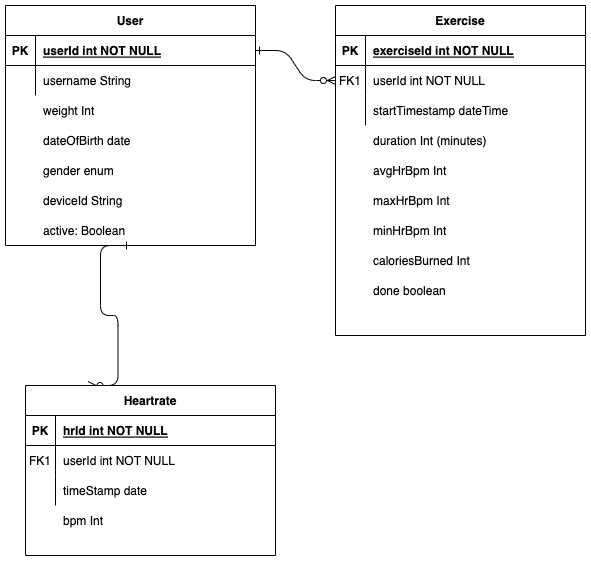
\includegraphics[width=0.8\textwidth]{diagrams/ham-entity.drawio.png}
    \caption{Entity class diagram}
    \label{fig:entity_diagram}
\end{figure}
{{\ttfamily \hyphenchar\the\font=`\-}
\autoref{fig:entity_diagram} visualizes the main entities and its relationship with each other inside the system. As illustrated by the diagram, the main entities in the system consist of \texttt{User}, \texttt{Exercise}, and \texttt{Heartrate}. 
Each \texttt{User} within the system has one to many relationship with both \texttt{Heartrate} and \texttt{Exercise} entities. These relationships represent the connection between a \texttt{User} and their corresponding \texttt{Heartrate} and \texttt{Exercise} records. 
Once the entities have been defined, the system's functionalities can now be discussed based on the identified use cases.
\par}


\subsubsection{Heart Rate Monitor}
\label{chap:hr_monitor_design}
A system sequence can now be defined as a result of analyzing the following user story:
\begin{quotation}
    \enquote{As a health-oriented user, I want to monitor my cardiovascular activity.} 
\end{quotation}

\begin{figure}[H]
    \centering
    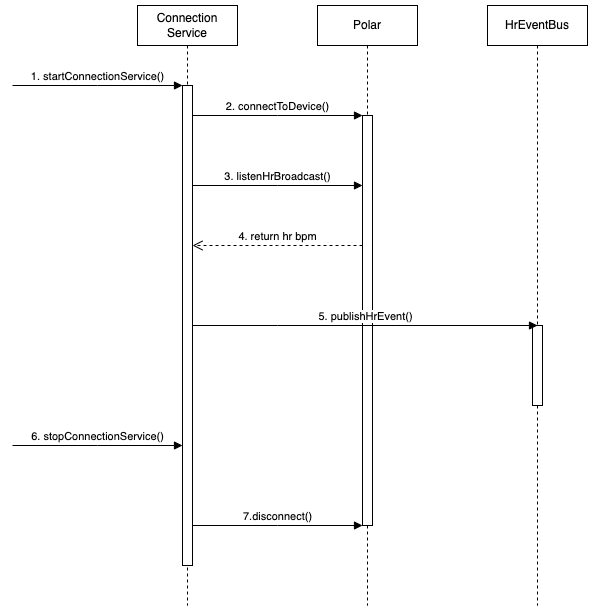
\includegraphics[width=0.9\textwidth]{diagrams/connection-service-onStart.drawio.png}
    \caption{Connection service sequence diagram}
    \label{fig:connection_diagram}
\end{figure}
Since one of the requirements is to monitor real-time heart rate, it is mandatory to establish connection to the heart rate sensor and handle the broadcasted heart rate data. The user should have a way to easily connect and disconnect from the device as desired.
The following sequence is visualized in \autoref{fig:connection_diagram} and it will be executed as a way to maintain connection to the BLE heart rate sensor and retrieve the heart rate data.
\begin{enumerate}
    \item A request to start the \texttt{ConnectionService} is received.
    \item The service initiates a bluetooth low energy connection to the heart rate sensor device.
    \item After the connection has been established, the \texttt{ConnectionService} listens to the heart rate data broadcasted by the heart rate sensor device.
    \item The broadcasted heart rate data is received.
    \item The service publishes an event containing the received heart rate data to the \texttt{HrEventBus}.
    \item A request to stop the \texttt{ConnectionService} is received.
    \item The service stops the connection with the heart rate sensor device.
\end{enumerate}

\subsubsection{Activity Monitor}
\label{chap:activity_monitor_design}
Based on the analysis of the following user story, a system sequence that outlines the sequence of actions and interactions within the system can now be established.
\begin{quotation}
    \enquote{As a physically active individuals, I want to track my current activity so that I can make adjustments to my physical activities.} 
\end{quotation}

\begin{figure}[H]
    \centering
    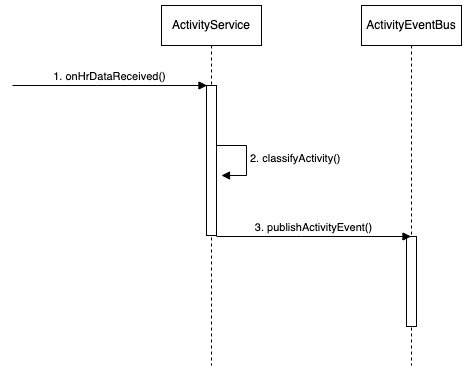
\includegraphics[width=0.8\textwidth]{diagrams/activity-monitor-seq.drawio.png}
    \caption{Activity service sequence diagram}
    \label{fig:activity_diagram}
\end{figure}

The following sequence in \autoref{fig:activity_diagram} illustrates the steps in monitoring the user's activity, which is one of the key use cases in the system:
\begin{enumerate}
    \item The \texttt{ActivityService} actively listens to the heart rate event broadcasted by the \texttt{ConnectionService} to the \texttt{HrEventBus}.
    \item Every time a heart rate event is received, the \texttt{ActivityService} classifies the user's current activity based on the user's current heart rate by using the formula mentioned in \autoref{chap:activity_intensity}
    \item Once the heart rate is classified, the service publishes an event containing the current activity.
\end{enumerate}

\subsubsection{Calculate Energy Expenditure}
\label{chap:burnedcalories_design}
Given that one of the requirements defined in the use cases of the system is to calculate burned calories or energy expenditure, it is necessary to implement a feature that enables the calculation of energy expenditure. 
Based on the formula mentioned in \autoref{chap:energy_expenditure}, it is required to specify the duration during which the calculation will be performed. 
To facilitate this, it is recommended to create a record of exercise. The exercise should hold the attributes needed for the calculation of the energy expenditure, for instance, the duration of the exercise and the average heart rate bpm.
Prior to initiating an exercise, it is necessary for the user to establish a connection with the heart rate sensor. This ensures the availability of real-time heart rate data, which is vital for accurate energy expenditure calculations during the exercise.

A system sequence can now be defined as a result of analyzing the following user story:
\begin{quotation}
    \enquote{As a fitness enthusiast, I want to know the number of calories burned in my exercises. This allows me to keep track of my progress and make adjustments to my exercises.} 
\end{quotation}

The following sequence is illustrated in \autoref{fig:start_exercise_diagram} and it is executed as a way to track the current exercise and calculate the energy expenditure:
\begin{enumerate}
    \item A request to start the exercise is received.
    \item The \texttt{ExerciseService} retrieves the active exercise from the repository, which is created and set active by the \texttt{ExerciseViewModel} when the user starts the exercise
    \item Active exercise is returned
    \item The \texttt{ExerciseService} actively listens to the heart rate event broadcasted by the \texttt{ConnectionService}.
    \item Heart rate event is retrieved.
    \item The \texttt{ExerciseService} processes active exercise. In this process, the attributes within the exercise such as average bpm and burned calories are calculated.
    \item The \texttt{ExerciseService} publishes an event containing the processed exercise.
    \item A request to stop the exercise is received.
    \item The active exercise is marked as done and processed.
    \item The completed exercise is persisted to the database by \texttt{ExerciseRepository}.
    \item The persisted exercise is returned.
    \item The \texttt{ExerciseService} publishes an event containing the completed exercise.
\end{enumerate}

\begin{figure}[H]
    \centering
    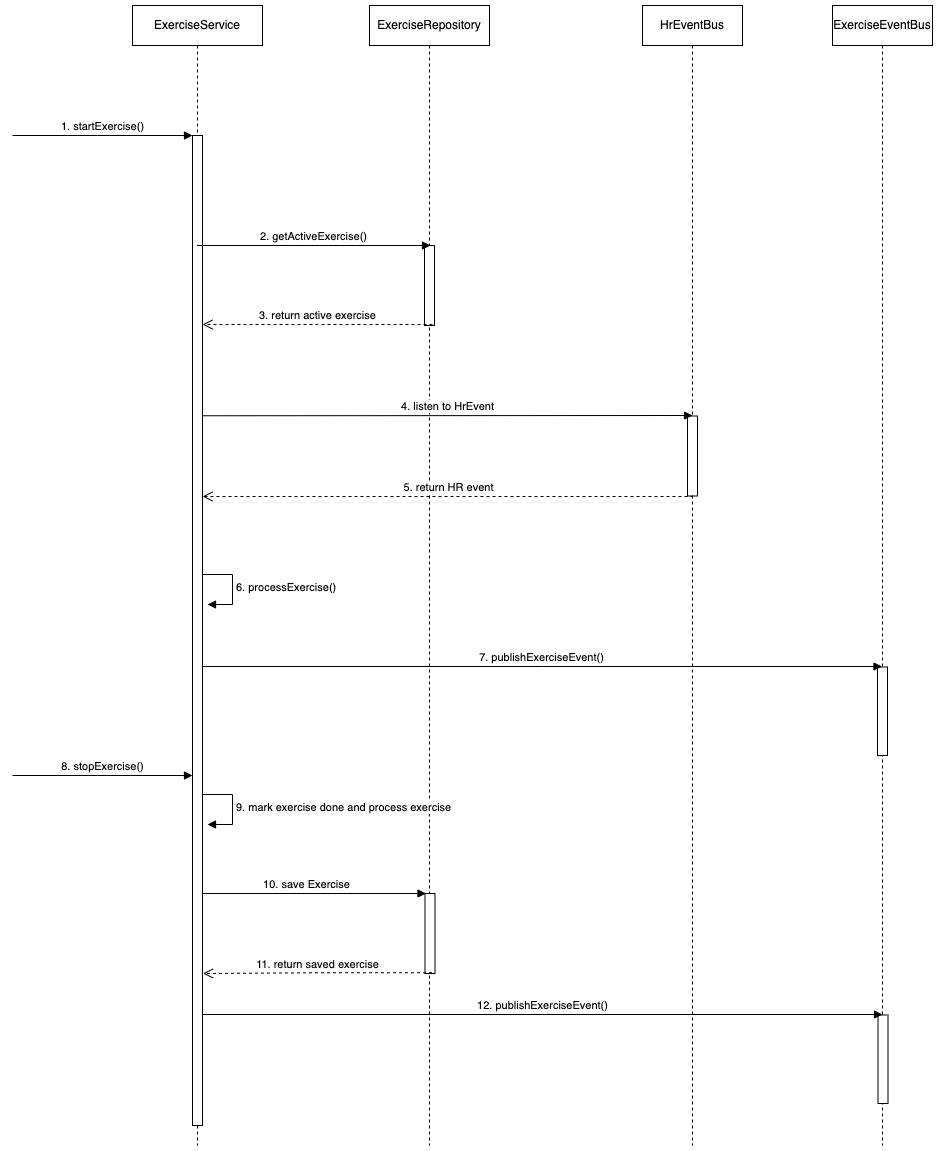
\includegraphics[width=1\textwidth]{diagrams/exercise-service-start.drawio.png}
    \caption{Exercise service on start and stop exercise sequence diagram}
    \label{fig:start_exercise_diagram}
\end{figure}

\subsubsection{Event Bus}
As the \emph{services} need to communicate with each other, it is very advantageous to implement an event bus based on the observable pattern described in Design Patterns \autocite{gamma1995design}. 
It involves using an event bus as a central hub for publishing and subscribing to events. Components can publish events to the bus without needing to know the receivers, and they can subscribe to specific types of events without knowing the publishers \autocite{turan2017}.
In the context of this project, there are three major event bus: \texttt{HrEventBus}, which handles events related to heart rate data; \texttt{ActivityEventBus}, responsible for managing events related to activity status; and lastly \texttt{ExerciseEventBus}, dedicated to handling exercise events.

\subsubsection{Profile Management}
According to the defined use cases in \autoref{chap:use_case}, it is essential to develop a functionality that enables users to manage their personal data. This functionality includes creating a new user profile, allowing users to modify their existing data, and lastly providing the users the capability to permanently delete their own data. These features will be implemented at the \emph{view model} level.
It will be discussed on \autoref{chap:viewmodel_design}



